\subsection{Pruebas y resultados}
	Para probar el funcionamiento del programa se utilizaron diferentes reglas con diferentes densidades de población, para observar el comportamiento de los mismos. Es importante señalar que todas las pruebas se hicieron con un $\tau=4$ y con diferentes funciones $\Phi$ además de solo iterar cerca de 100 veces.

	\subsubsection{Regla: 2 7 4 6. Densidad: 20\%}
	Como se puede observar en la figura \ref{fig:golm1} esta regla termina por llenar la mayor parte espacio con una malla de unos y ceros.
	\begin{figure}[H]
		\begin{center}
			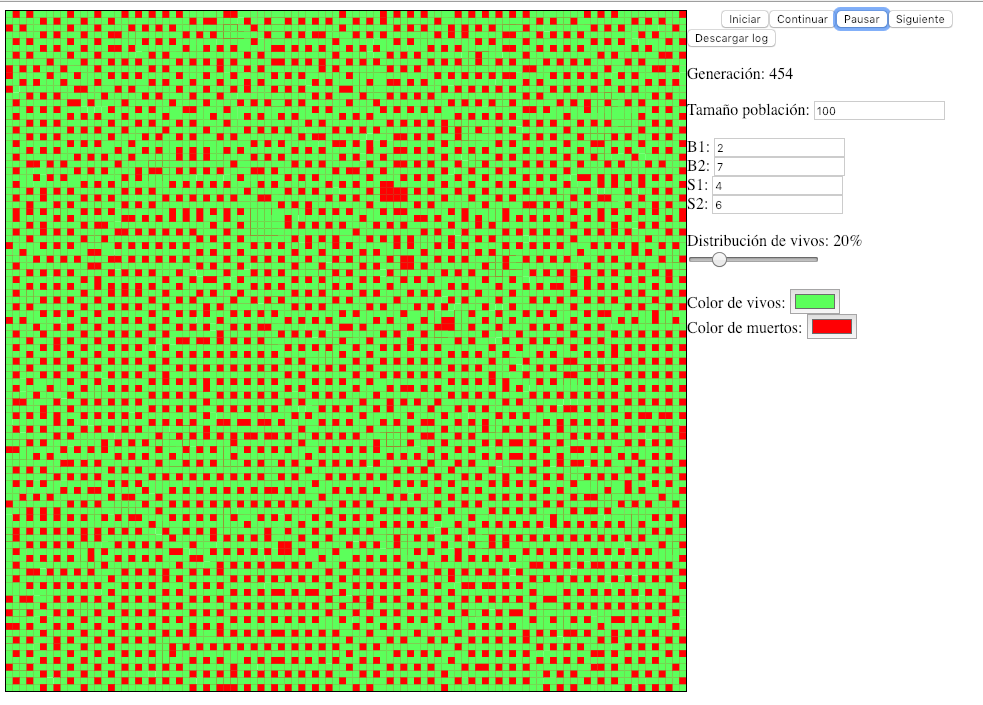
\includegraphics[scale=.3]{GOLM/img/regla2746-0.png}
			\caption{Resultado de iterar 100 veces sin memoria}
			\label{fig:golm1}
		\end{center}
	\end{figure}

	Como se puede observar en la figura \ref{fig:golm2}, el comportamiento de este autómata usando la función de máximo es muy similar a su comportamiento normal.
	\begin{figure}[H]
		\begin{center}
			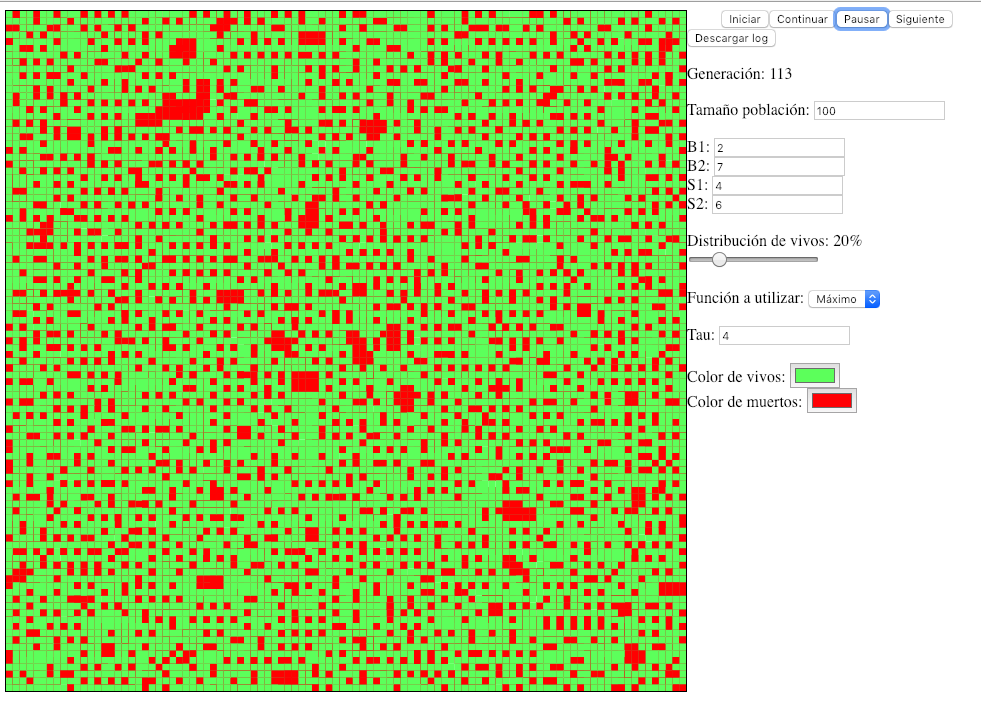
\includegraphics[scale=.3]{GOLM/img/regla2746-1.png}
			\caption{Resultado de iterar usando función de máximo}
			\label{fig:golm2}
		\end{center}
	\end{figure}

	De igual manera, la matriz auxiliar se comporta similar, sin embargo, se distingue que está tiene menos células muertas.
	\begin{figure}[H]
		\begin{center}
			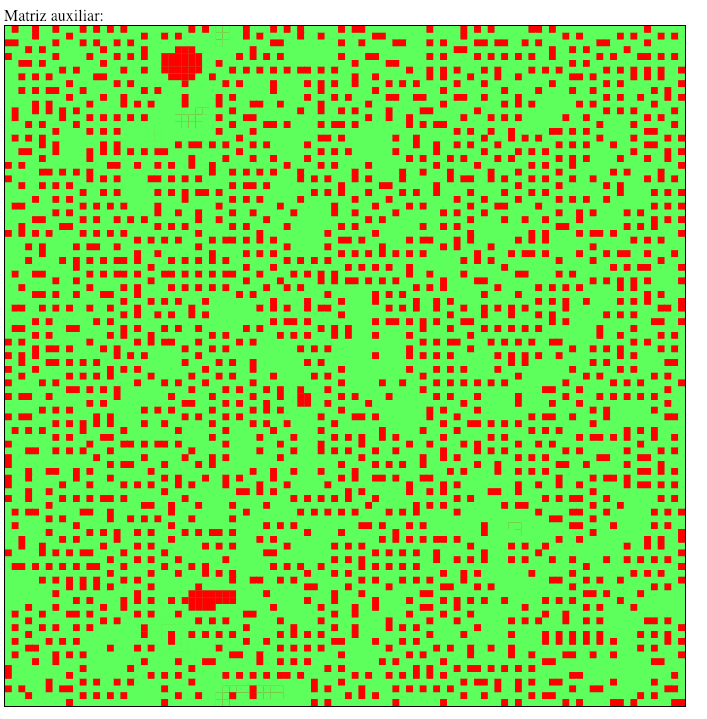
\includegraphics[scale=.3]{GOLM/img/regla2746-1-1.png}
			\caption{Matriz auxiliar}
			\label{fig:golm3}
		\end{center}
	\end{figure}

	Sin embargo, en la figura \ref{fig:golm4} podemos observar como es que la función de mínimo se comporta distinto, ya que pareciera que esta generando algunos patrones dentro de la malla que parecieran repetirse.
	\begin{figure}[H]
		\begin{center}
			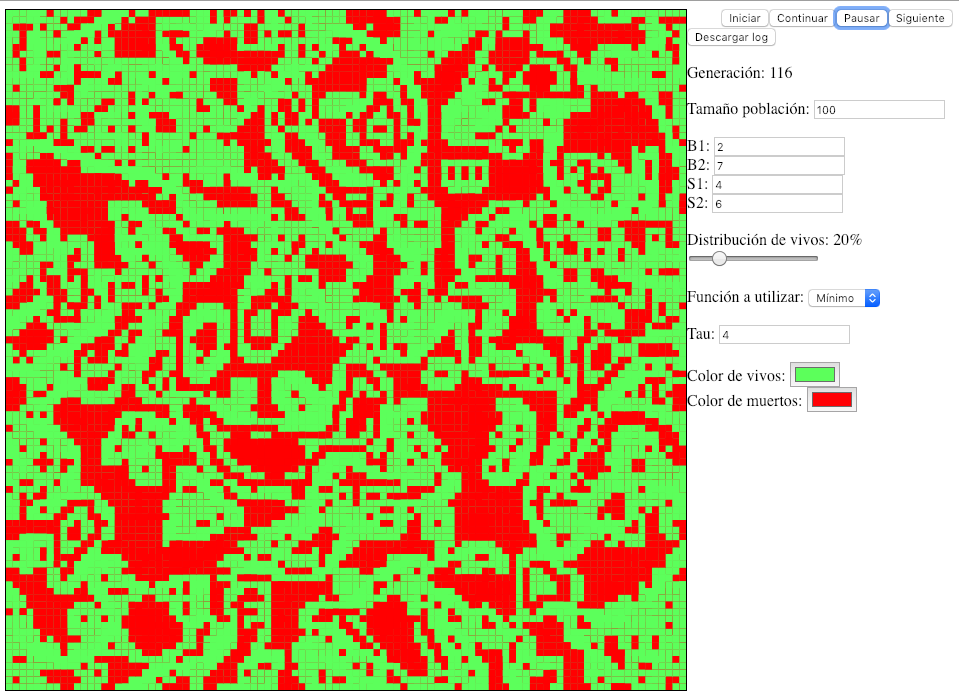
\includegraphics[scale=.3]{GOLM/img/regla2746-2.png}
			\caption{Resultado de iterar usando función de mínimo}
			\label{fig:golm4}
		\end{center}
	\end{figure}

	La matriz auxiliar de esta, solo aparenta estar cambiando de colores.
	\begin{figure}[H]
		\begin{center}
			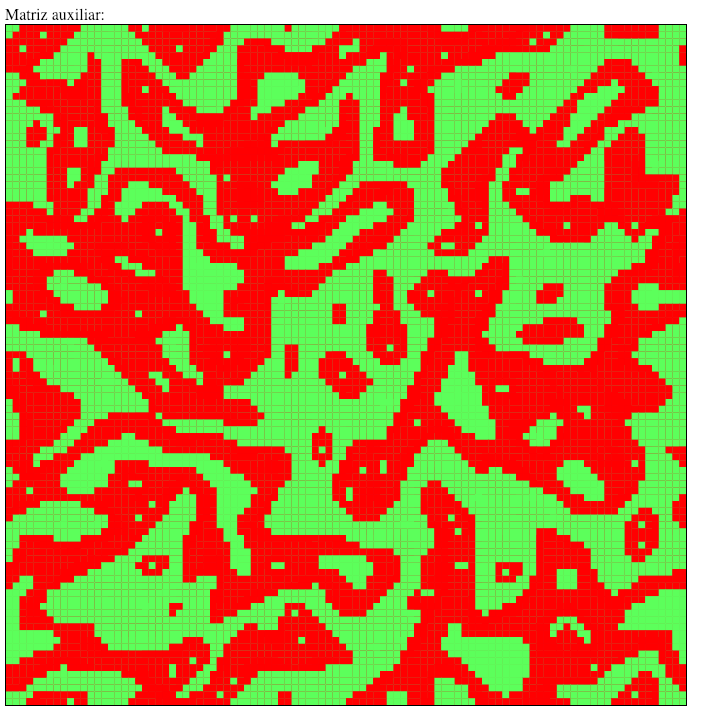
\includegraphics[scale=.3]{GOLM/img/regla2746-2-1.png}
			\caption{Matriz auxiliar}
			\label{fig:golm5}
		\end{center}
	\end{figure}

	Tiene un comportamiento similar a la de máximo, sin embargo, tiene más ``huecos'' que la otra.
	\begin{figure}[H]
		\begin{center}
			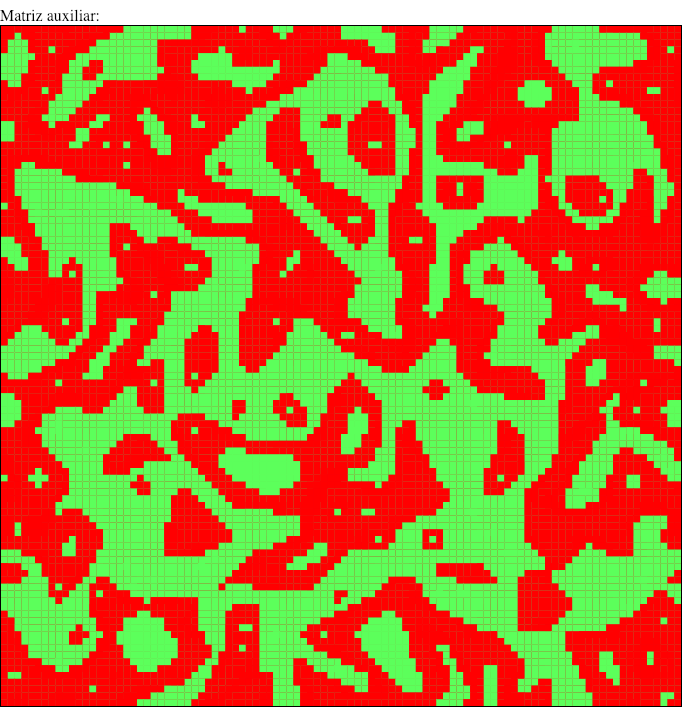
\includegraphics[scale=.3]{GOLM/img/regla2746-3.png}
			\caption{Resultado de iterar usando función de paridad}
			\label{fig:golm6}
		\end{center}
	\end{figure}

	\begin{figure}[H]
		\begin{center}
			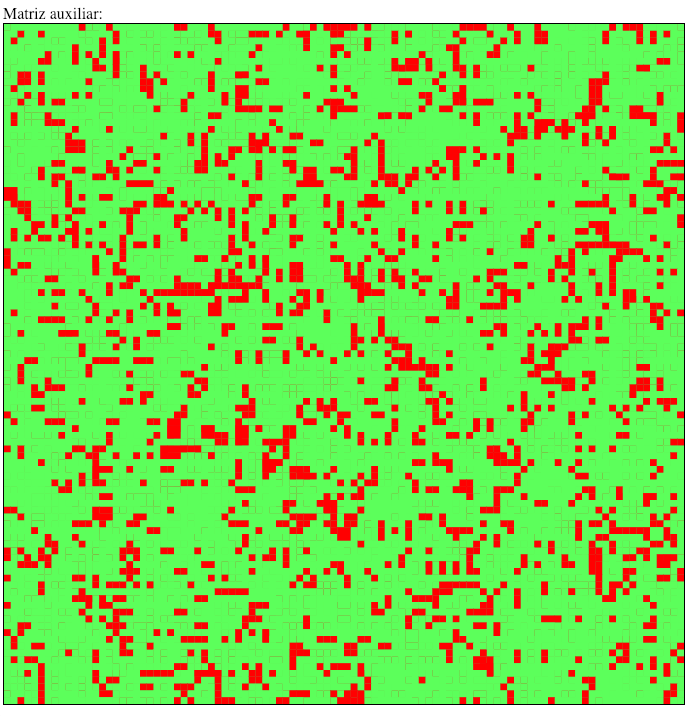
\includegraphics[scale=.3]{GOLM/img/regla2746-3-1.png}
			\caption{Matriz auxiliar}
			\label{fig:golm7}
		\end{center}
	\end{figure}



	\subsubsection{Regla: 3 6 3 4 (Cruz en el centro)}
	Como se puede observar en la figura \ref{fig:golm8} esta regla permite formar mosaicos los cuales van creciendo de tamaño, para lograr esto, la distribución se coloco en cero y se agregaron 7 cuadros en forma de cruz al centro (esto sin usar memoria).
	\begin{figure}[H]
		\begin{center}
			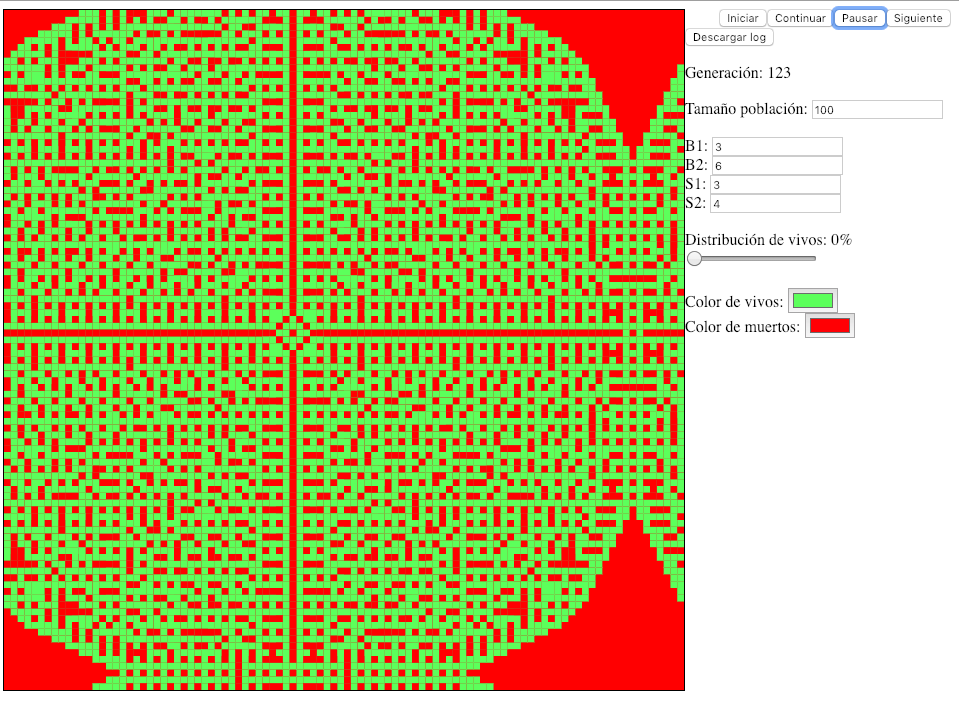
\includegraphics[scale=.3]{GOLM/img/regla3634-0.png}
			\caption{Resultado de poner una cruz al centro}
			\label{fig:golm8}
		\end{center}
	\end{figure}

	En la figura \ref{fig:golm9}, el comportamiento de este autómata usando la función de mínimo es muy similar a su comportamiento sin memoria, sin embargo, el mosaico formado es distinto.
	\begin{figure}[H]
		\begin{center}
			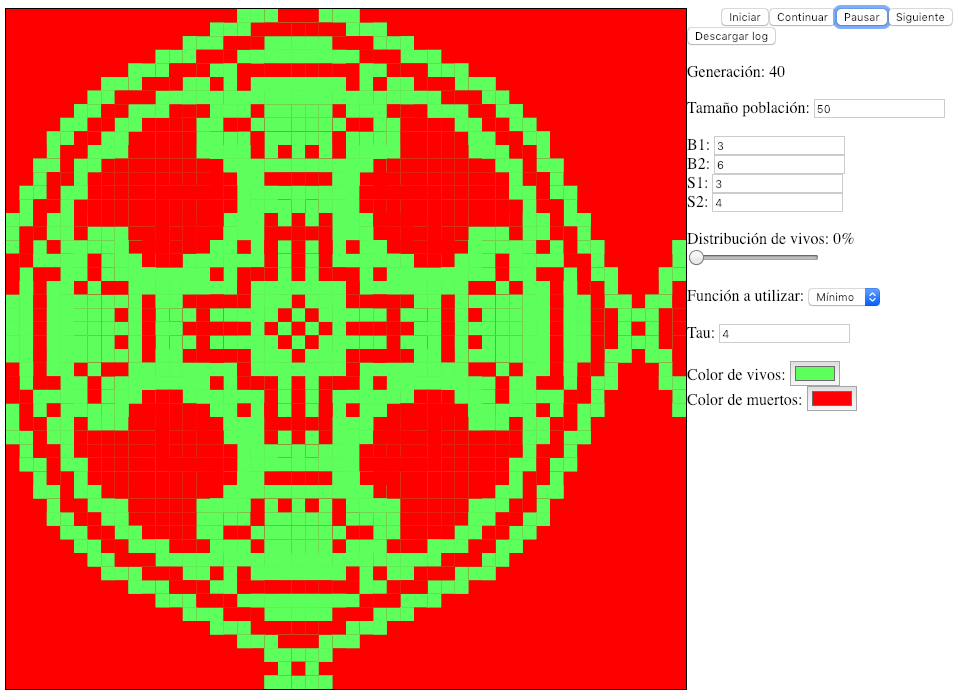
\includegraphics[scale=.3]{GOLM/img/regla3634-1.png}
			\caption{Resultado de iterar usando función de mínimo}
			\label{fig:golm9}
		\end{center}
	\end{figure}

	De igual manera, la matriz auxiliar forma mosaicos, pero con al diferencia, que las células que están vivas en máximo están muertas en auxiliar y viceversa.
	\begin{figure}[H]
		\begin{center}
			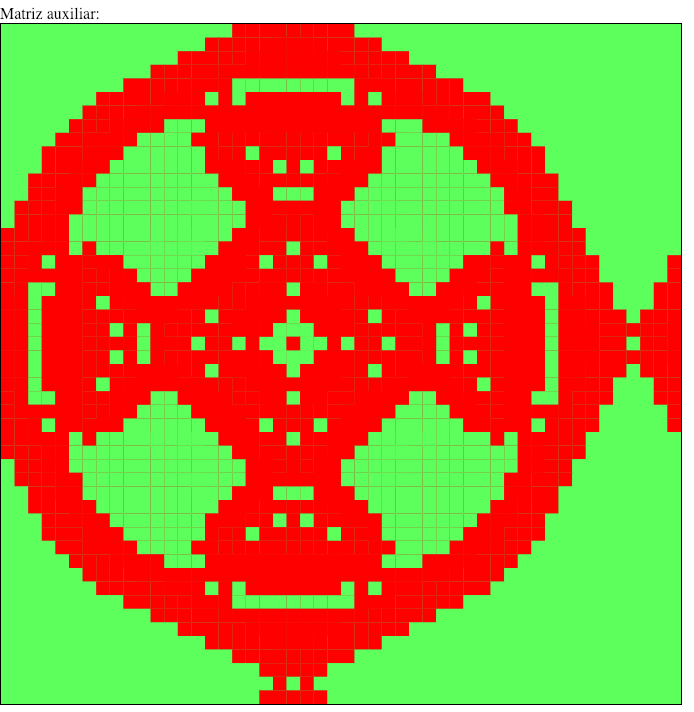
\includegraphics[scale=.3]{GOLM/img/regla3634-1-1.png}
			\caption{Matriz auxiliar}
			\label{fig:golm10}
		\end{center}
	\end{figure}


	Al aplica la función de máximo el resultado es el mismo que al usar mínimo.
	\begin{figure}[H]
		\begin{center}
			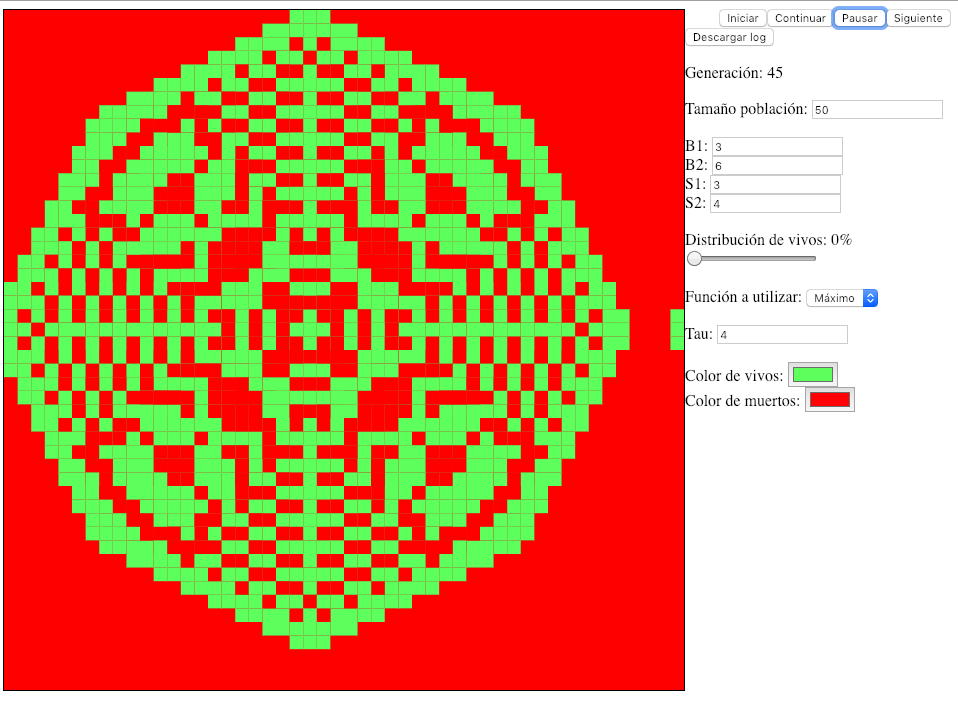
\includegraphics[scale=.3]{GOLM/img/regla3634-2.png}
			\caption{Resultado de iterar usando función de máximo}
			\label{fig:golm11}
		\end{center}
	\end{figure}

	Sin embargo, la matriz auxiliar cambia y no es igual a la de mínimo, es otro mosaico distinto.
	\begin{figure}[H]
		\begin{center}
			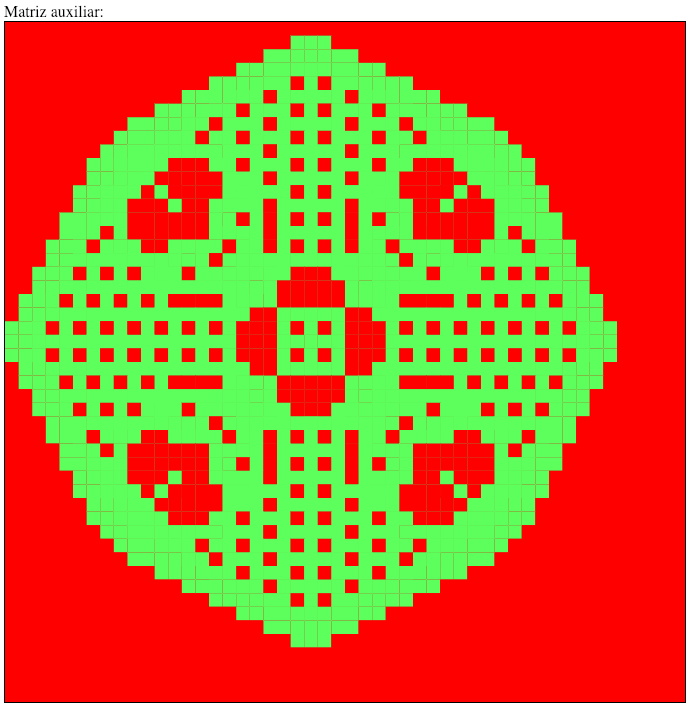
\includegraphics[scale=.3]{GOLM/img/regla3634-2-1.png}
			\caption{Matriz auxiliar}
			\label{fig:golm12}
		\end{center}
	\end{figure}


	Finalmente, al aplica la función paridad, podemos observar otro mosaico muy distinto a los anteriores, ya que está tarda más generaciones que los demás en expandirse.
	\begin{figure}[H]
		\begin{center}
			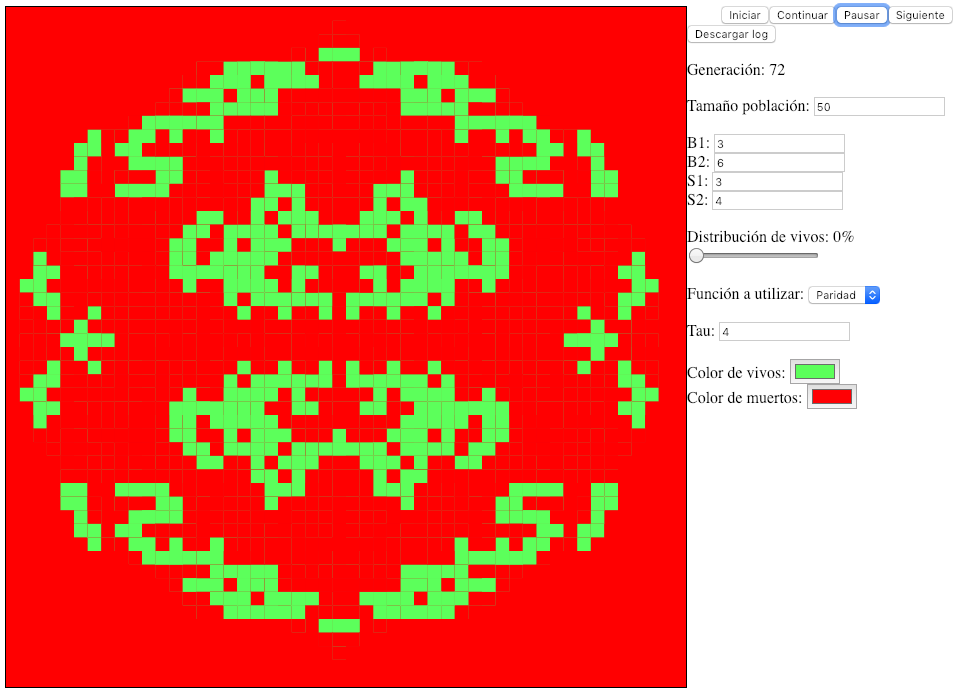
\includegraphics[scale=.3]{GOLM/img/regla3634-3.png}
			\caption{Resultado de iterar usando función de paridad}
			\label{fig:golm13}
		\end{center}
	\end{figure}

	Al igual que en mínimo, la matriz auxiliar de la función paridad intercambia los colores con esta.
	\begin{figure}[H]
		\begin{center}
			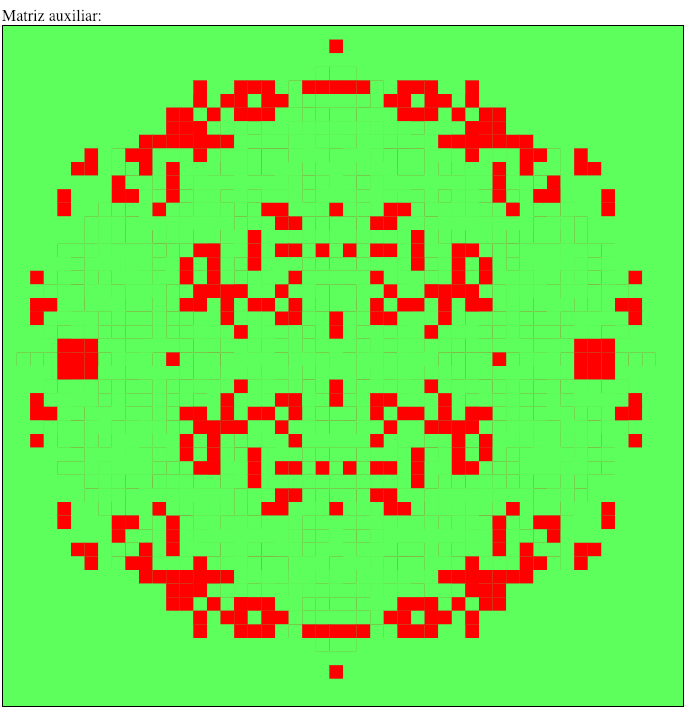
\includegraphics[scale=.3]{GOLM/img/regla3634-3-1.png}
			\caption{Matriz auxiliar}
			\label{fig:golm14}
		\end{center}
	\end{figure}



	\subsubsection{Regla: 1 6 1 6. Densidad: 10\%}
	Como se puede observar en la figura \ref{fig:golm15} esta regla forma una especie de laberinto que va cambiando pero en determinada generación, este patrón empieza a repetirse y oscila cada dos generaciones. (Sin memoria)
	\begin{figure}[H]
		\begin{center}
			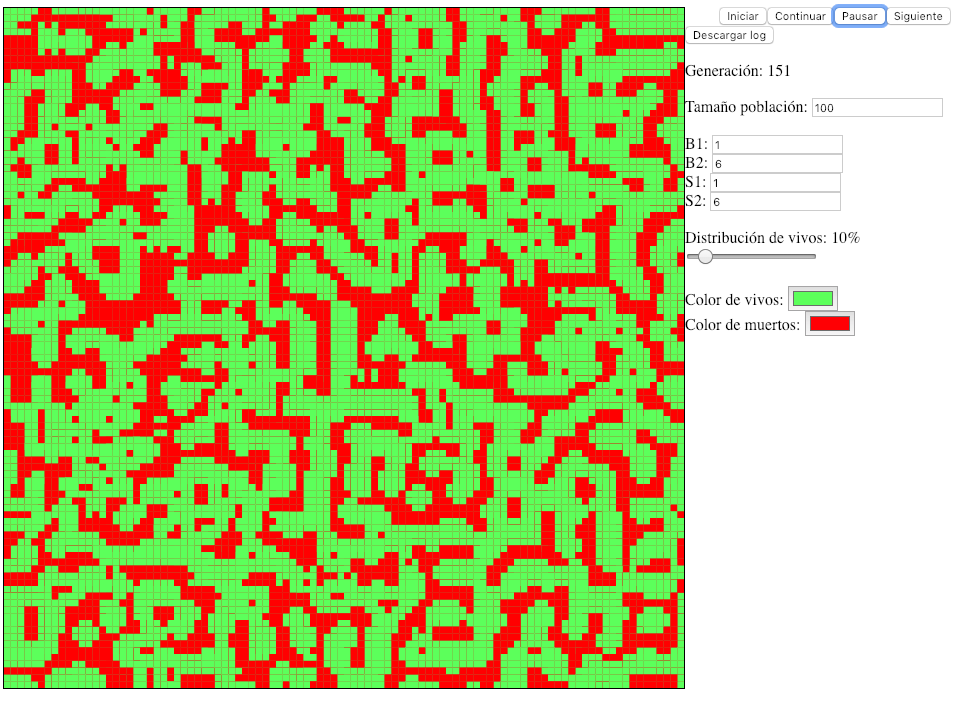
\includegraphics[scale=.3]{GOLM/img/regla1616-0.png}
			\caption{Resultado de iterar 100 veces sin memoria}
			\label{fig:golm15}
		\end{center}
	\end{figure}

	En la figura \ref{fig:golm16}, el comportamiento de este autómata usando la función de máximo es un tanto similar a su comportamiento normal dado que llega el momento que empiezan a oscilar sus formas y se repiten los mismo patrones, sin embargo, la forma que se consigue es distinta, ya que ``el laberinto'' formado se compone de paredes más delgadas.
	\begin{figure}[H]
		\begin{center}
			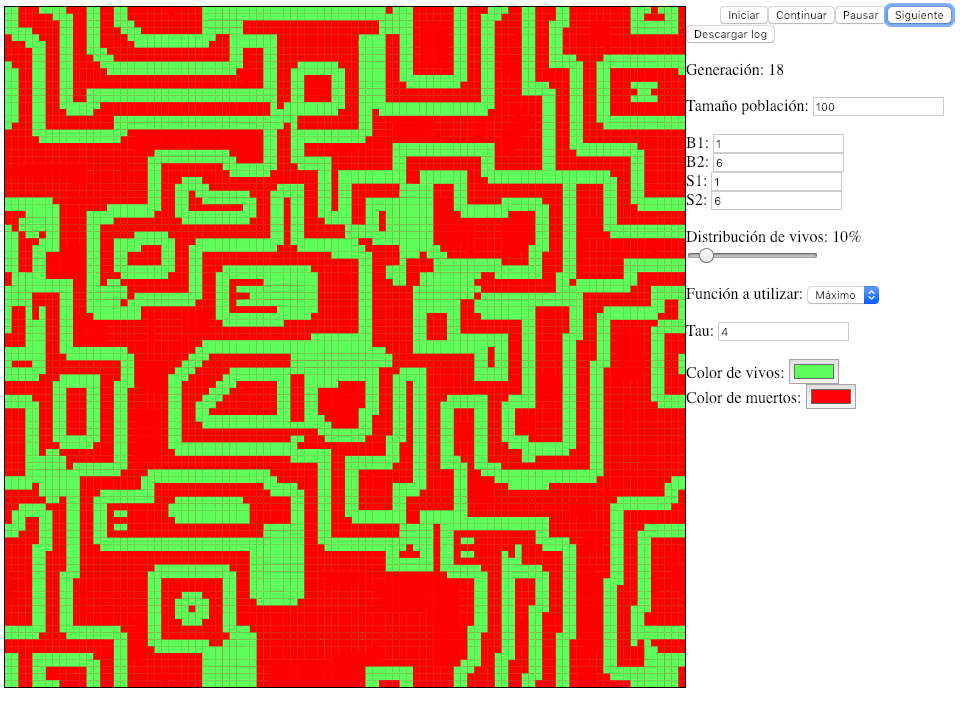
\includegraphics[scale=.3]{GOLM/img/regla1616-1.png}
			\caption{Resultado de iterar usando función de máximo}
			\label{fig:golm16}
		\end{center}
	\end{figure}

	La matriz auxiliar del autómata anterior, forma igualmente un ``laberinto'' sin embargo sus paredes son más grusas y además, también tiene un patrón que se repite eternamente.
	\begin{figure}[H]
		\begin{center}
			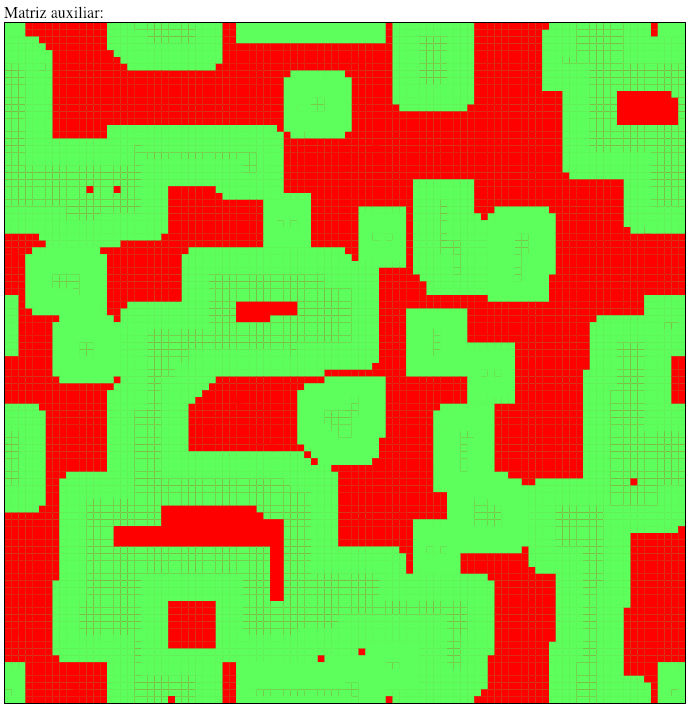
\includegraphics[scale=.3]{GOLM/img/regla1616-1-1.png}
			\caption{Matriz auxiliar}
			\label{fig:golm17}
		\end{center}
	\end{figure}

	Sin embargo, en la figura \ref{fig:golm18} podemos observar el autómata con la función mínimo, de igual manera oscila repitiendo ciertos patrones solo que su periodo es mayor, ya que le toma más generaciones regresar a una forma que con máximo.
	\begin{figure}[H]
		\begin{center}
			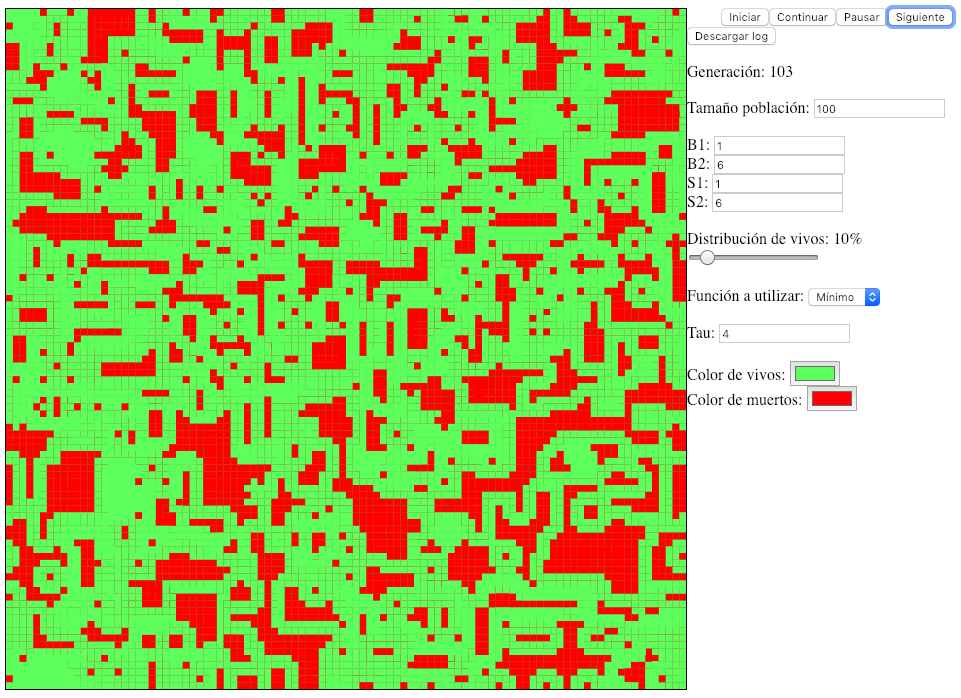
\includegraphics[scale=.3]{GOLM/img/regla1616-2.png}
			\caption{Resultado de iterar usando función de mínimo}
			\label{fig:golm18}
		\end{center}
	\end{figure}

	La matriz auxiliar de igual forma oscila con la poca población que tiene.
	\begin{figure}[H]
		\begin{center}
			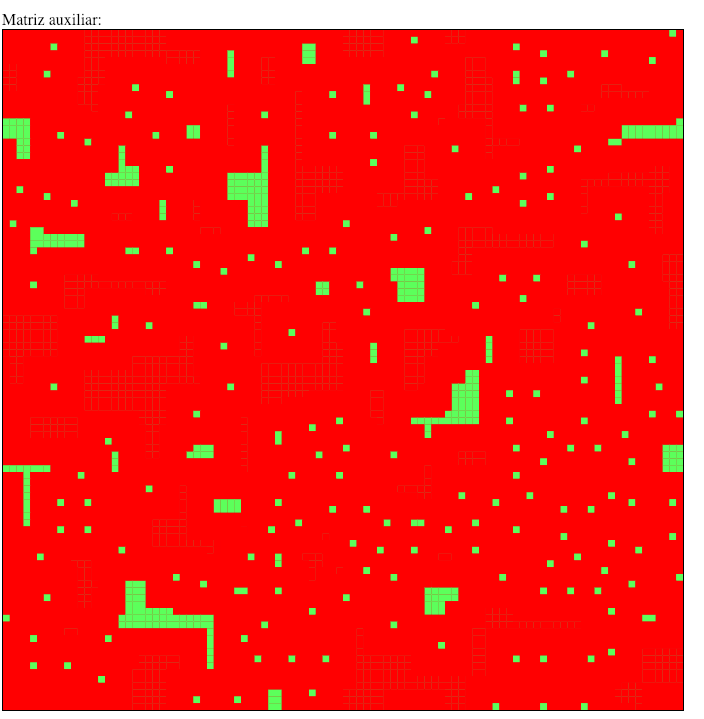
\includegraphics[scale=.3]{GOLM/img/regla1616-2-1.png}
			\caption{Matriz auxiliar}
			\label{fig:golm19}
		\end{center}
	\end{figure}

	En la siguiente figura, se observa el resultado de usar la función de paridad, al igual que las anteriores funciones, se repiten los patrones en la malla de forma cíclica.
	\begin{figure}[H]
		\begin{center}
			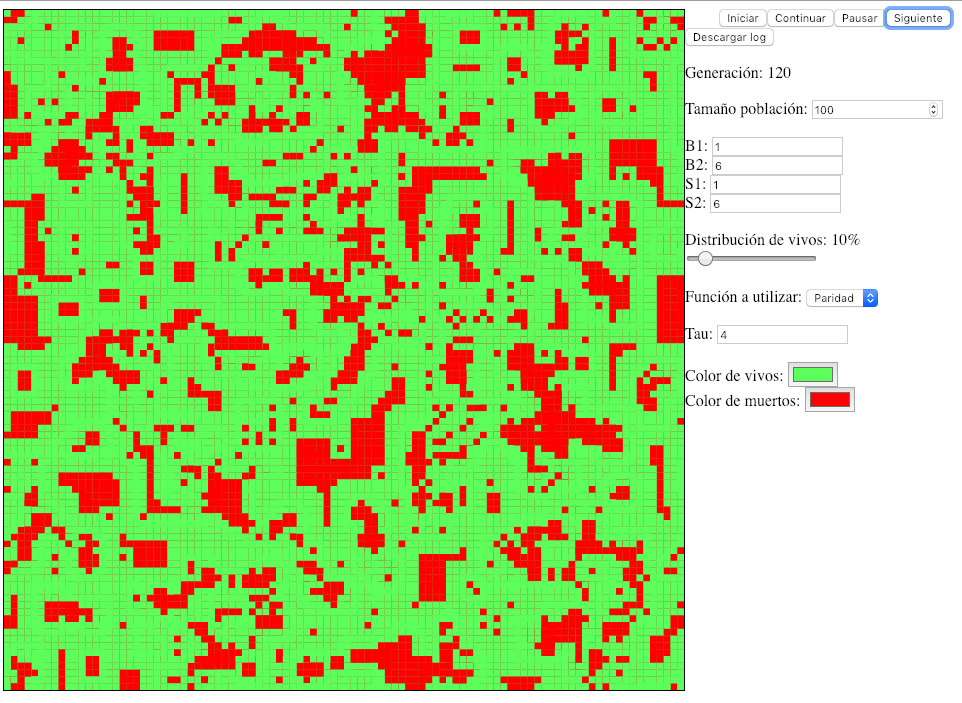
\includegraphics[scale=.3]{GOLM/img/regla1616-3.png}
			\caption{Resultado de iterar usando función de paridad}
			\label{fig:golm20}
		\end{center}
	\end{figure}

	Cabe señalar, que paridad tiene algo interesante, ya que hay que observar su matriz auxiliar para notar que tiene una forma bastante particular.
	\begin{figure}[H]
		\begin{center}
			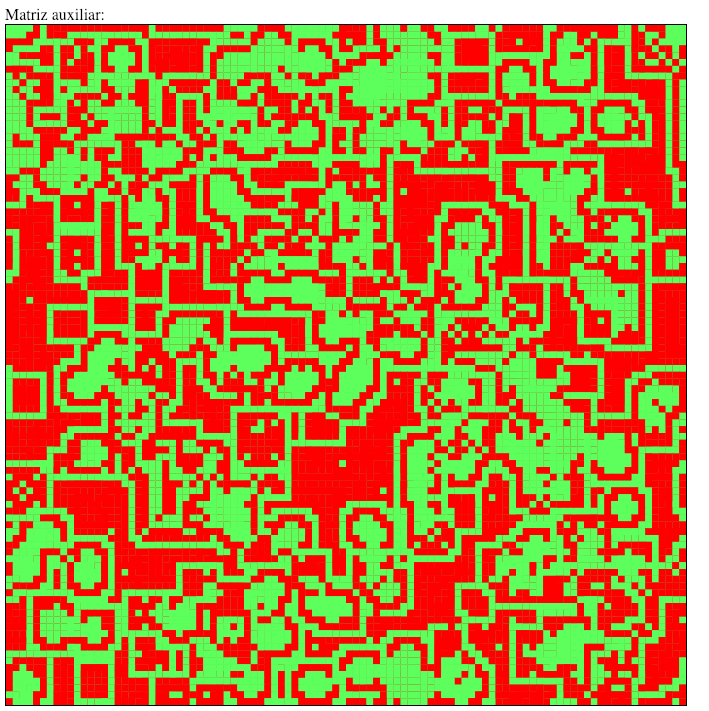
\includegraphics[scale=.3]{GOLM/img/regla1616-3-1.png}
			\caption{Matriz auxiliar}
			\label{fig:golm21}
		\end{center}
	\end{figure}




	\subsubsection{Regla: 3 3 1 8. Densidad: 10\%}
	Como se puede observar en la figura \ref{fig:golm22} esta regla después del paso de algunas generaciones queda estancada y no sufre cambio alguno (salvo alguno pequeño que no llega a deformarlo), la población se mantiene oscilando entre un limite mayor y un límite menor.
	\begin{figure}[H]
		\begin{center}
			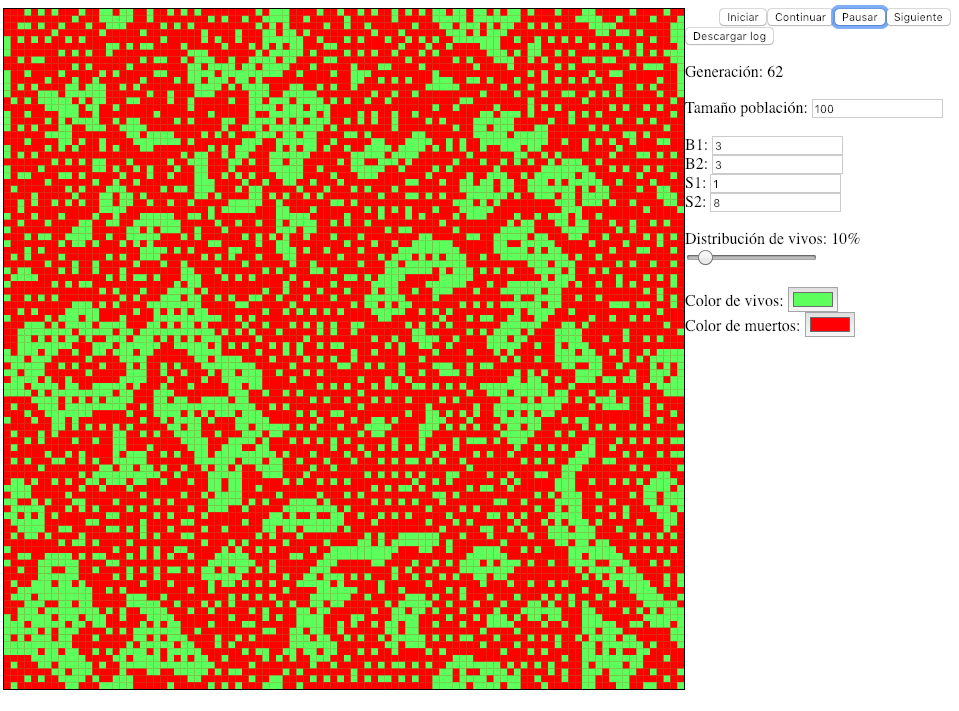
\includegraphics[scale=.3]{GOLM/img/regla3318-0.png}
			\caption{Resultado de iterar 100 veces sin memoria}
			\label{fig:golm22}
		\end{center}
	\end{figure}

	En la figura \ref{fig:golm23}, el comportamiento de este autómata usando la función de máximo es distinta a su comportamiento normal, ya que esta función provoca que el autómata oscile repitiendo formas cada cierto número de generaciones, y dentro de este se forman cuadrados y rectángulos los cuales a su vez dentro tienen otras formas como mosaicos.
	\begin{figure}[H]
		\begin{center}
			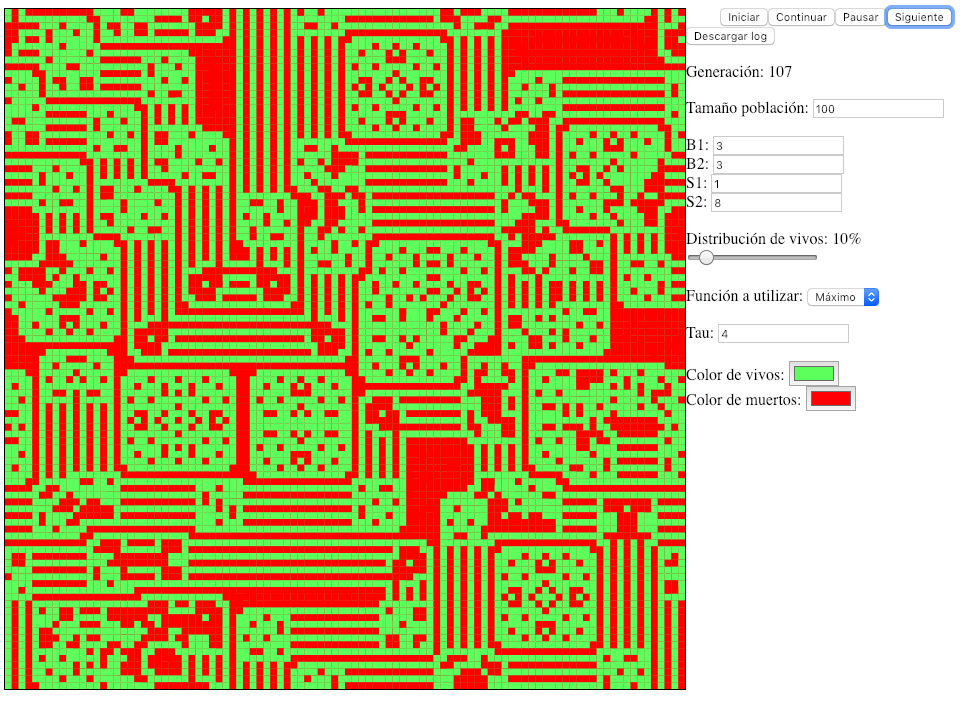
\includegraphics[scale=.3]{GOLM/img/regla3318-1.png}
			\caption{Resultado de iterar usando función de máximo}
			\label{fig:golm23}
		\end{center}
	\end{figure}

	La matriz auxiliar del autómata anterior, tiene una forma bastante peculiar, ya que recuerda a un rompecabezas, debido a que tiene secciones muy definidas dentro de él las cuales no se tocan ni superponen.
	\begin{figure}[H]
		\begin{center}
			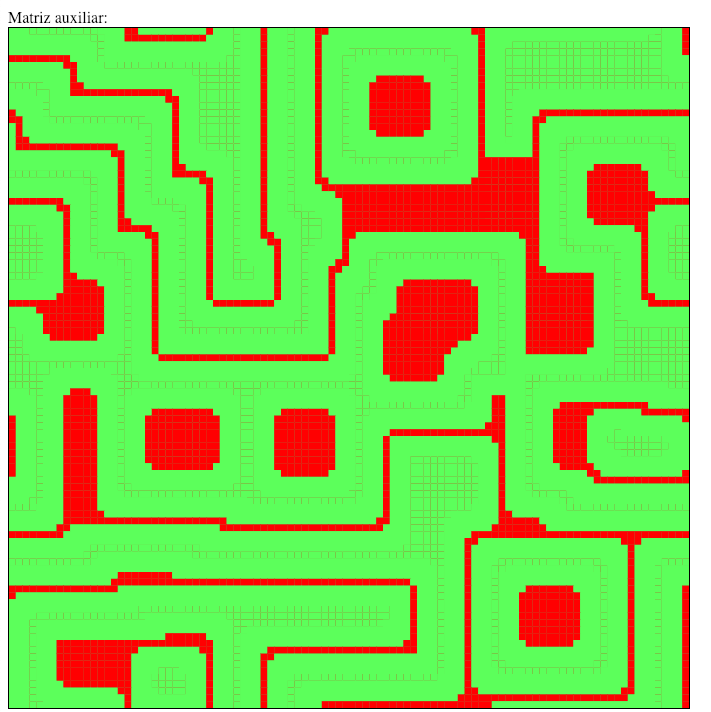
\includegraphics[scale=.3]{GOLM/img/regla3318-1-1.png}
			\caption{Matriz auxiliar}
			\label{fig:golm24}
		\end{center}
	\end{figure}


	Al aplicar la función de mínimo, el autómata de igual forma pareciera que se encuentra oscilando y de cierta forma recuerda a un circuito eléctrico (a una placa mejor dicho).
	\begin{figure}[H]
		\begin{center}
			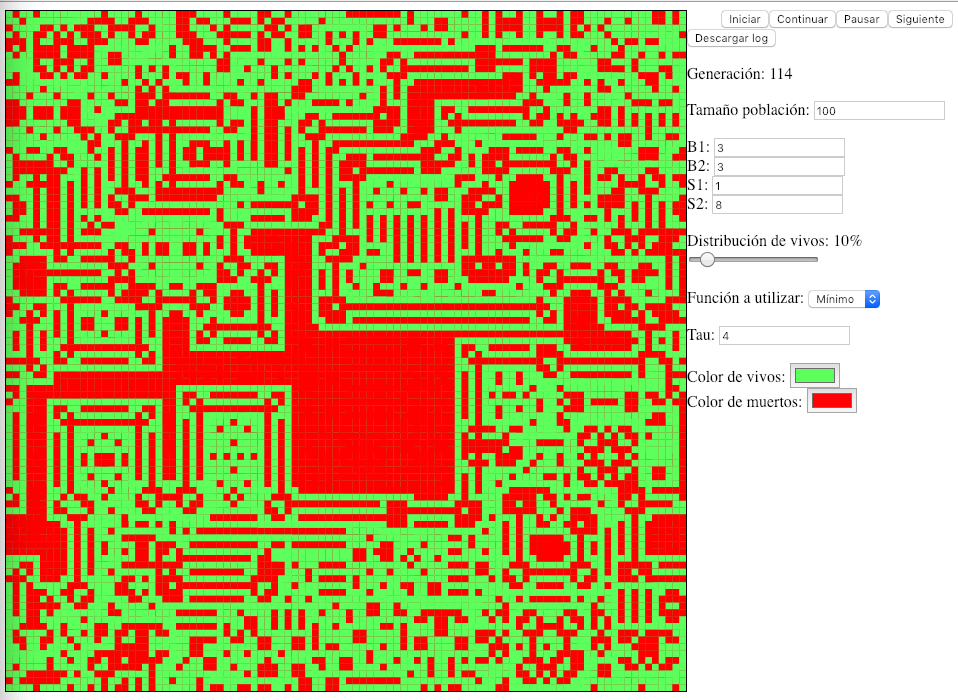
\includegraphics[scale=.3]{GOLM/img/regla3318-2.png}
			\caption{Resultado de iterar usando función de mínimo}
			\label{fig:golm25}
		\end{center}
	\end{figure}

	La matriz auxiliar de igual manera oscila, pero con una población mucho menor.
	\begin{figure}[H]
		\begin{center}
			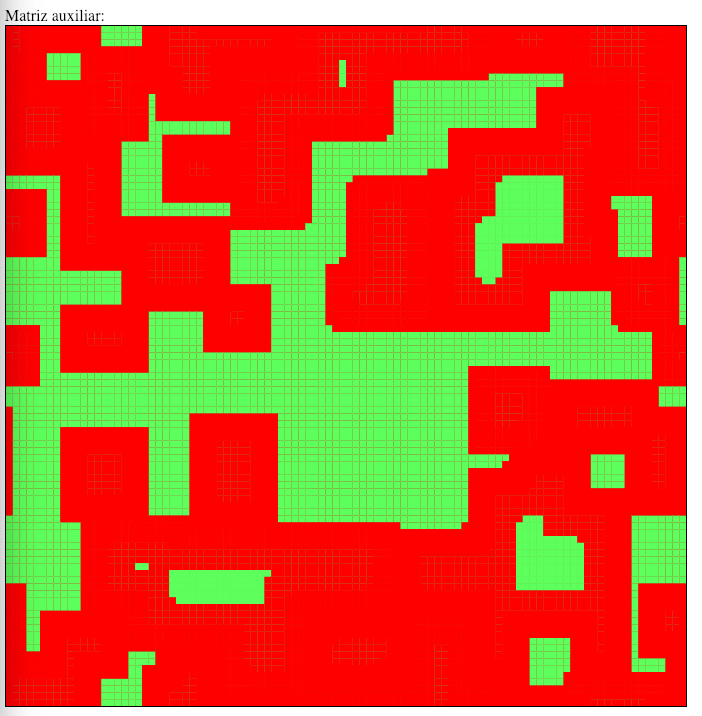
\includegraphics[scale=.3]{GOLM/img/regla3318-2-1.png}
			\caption{Matriz auxiliar}
			\label{fig:golm26}
		\end{center}
	\end{figure}

	En la siguiente figura, se observa el resultado de usar la función de paridad, la población no desciende mucho en este caso y pareciera se mantiene constante.
	\begin{figure}[H]
		\begin{center}
			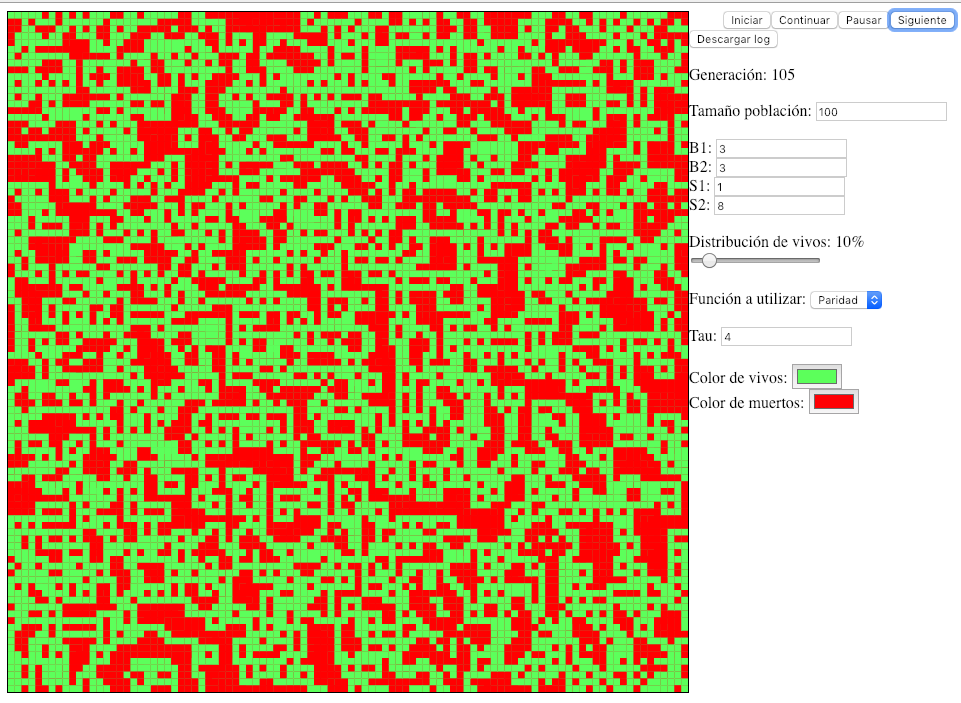
\includegraphics[scale=.3]{GOLM/img/regla3318-3.png}
			\caption{Resultado de iterar usando función de paridad}
			\label{fig:golm27}
		\end{center}
	\end{figure}

	la matriz auxiliar tiene una gran cantidad de población la cual también varia muy poco. Parece ser que paridad es la función más estable para este autómata.
	\begin{figure}[H]
		\begin{center}
			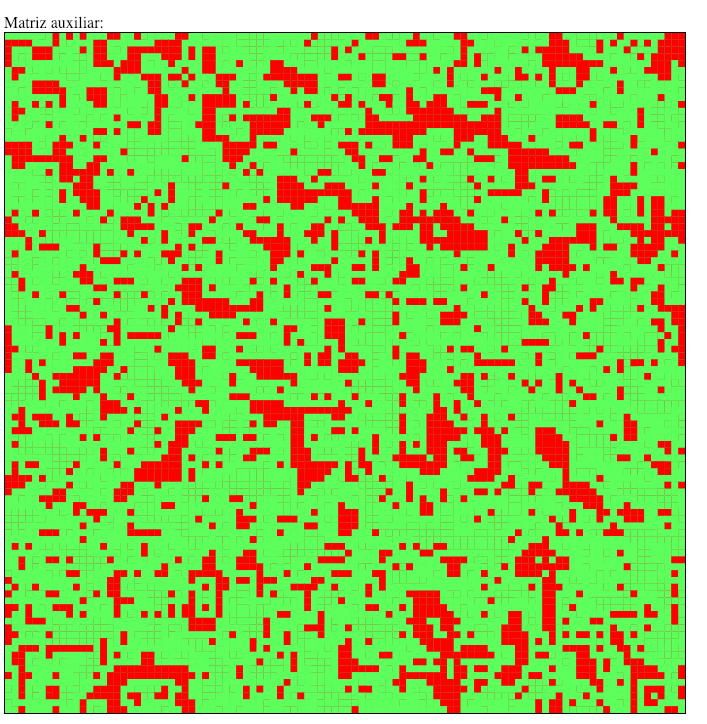
\includegraphics[scale=.3]{GOLM/img/regla3318-3-1.png}
			\caption{Matriz auxiliar}
			\label{fig:golm28}
		\end{center}
	\end{figure}



	\subsubsection{Regla: 3 3 1 7. Línea en el centro de 7 cuadros}
	Como se puede observar en la figura \ref{fig:golm29}, esta regla provoca mosaicos que se repiten indeterminadamente (sin memoria),para esto, se colocaron 7 cuadros en el centro en línea horizontal.
	\begin{figure}[H]
		\begin{center}
			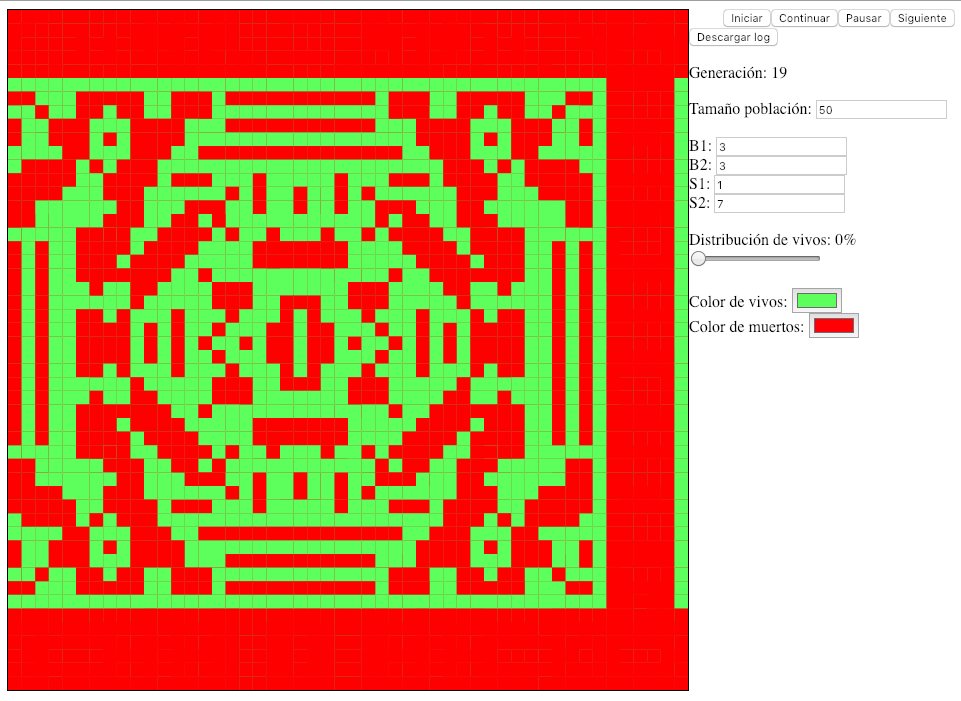
\includegraphics[scale=.3]{GOLM/img/regla3317-0.png}
			\caption{Resultado de iterar 20 veces sin memoria}
			\label{fig:golm29}
		\end{center}
	\end{figure}

	En la figura \ref{fig:golm30}, se muestra el comportamiento de este autómata al aplicar la función de máximo, el cual forma mosaicos, pero tienen una forma diferente a los que produce ``normal'', ya que ahora estos en el centro tienen un rectángulo.
	\begin{figure}[H]
		\begin{center}
			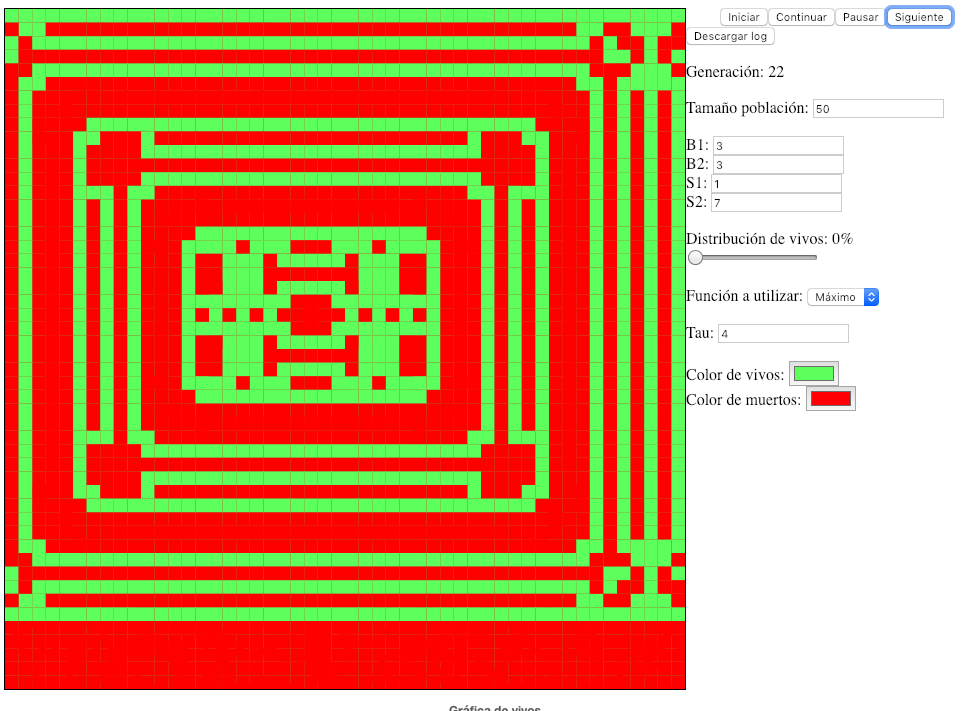
\includegraphics[scale=.3]{GOLM/img/regla3317-1.png}
			\caption{Resultado de iterar usando función de máximo}
			\label{fig:golm30}
		\end{center}
	\end{figure}

	De igual forma, la matriz auxiliar, forma un mosaico, pero este es mucho menos vistoso ya que tiene líneas muy gruesas.
	\begin{figure}[H]
		\begin{center}
			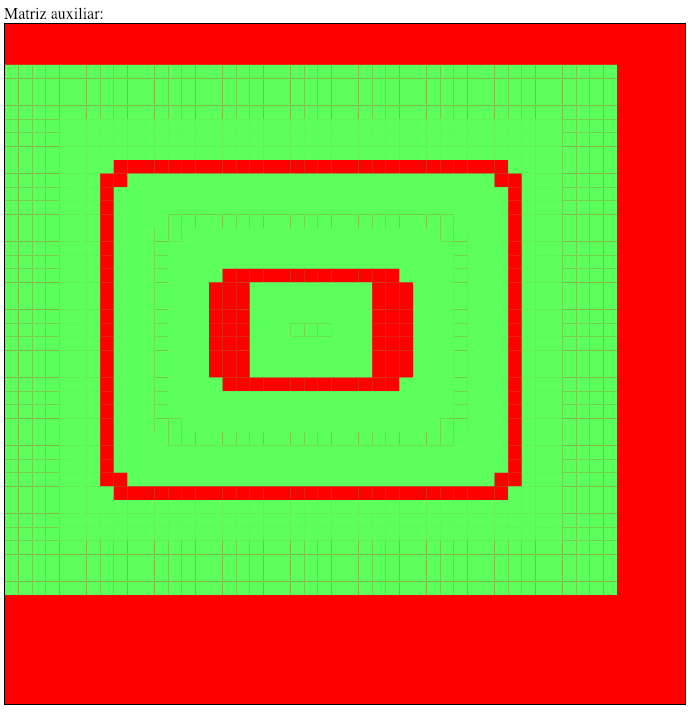
\includegraphics[scale=.3]{GOLM/img/regla3317-1-1.png}
			\caption{Matriz auxiliar}
			\label{fig:golm31}
		\end{center}
	\end{figure}


	Al aplicar la función de mínimo, el autómata después de casi 80 generaciones, empezó a formar líneas las cuales son paralelas y abarcan el espacio de todo el canvas. Este es el primer autómata que veo hace eso.
	\begin{figure}[H]
		\begin{center}
			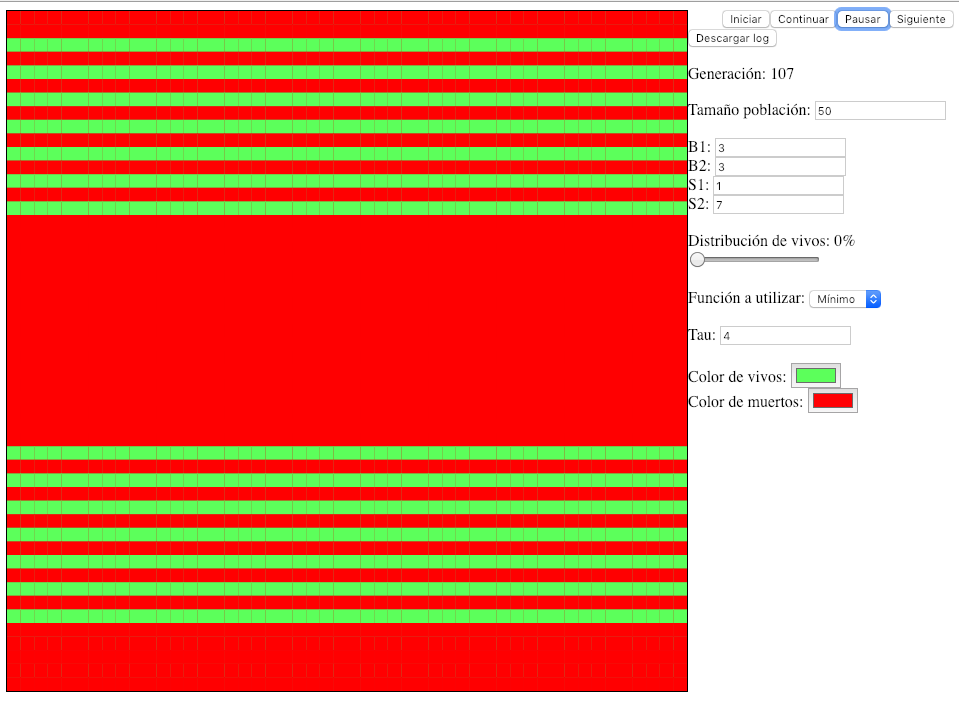
\includegraphics[scale=.3]{GOLM/img/regla3317-2.png}
			\caption{Resultado de iterar usando función de mínimo}
			\label{fig:golm32}
		\end{center}
	\end{figure}

	La matriz auxiliar del autómata anterior, de igual forma cuenta con líneas, solo que estás son mucho mas gruesas, y diden el espacio en tres.
	\begin{figure}[H]
		\begin{center}
			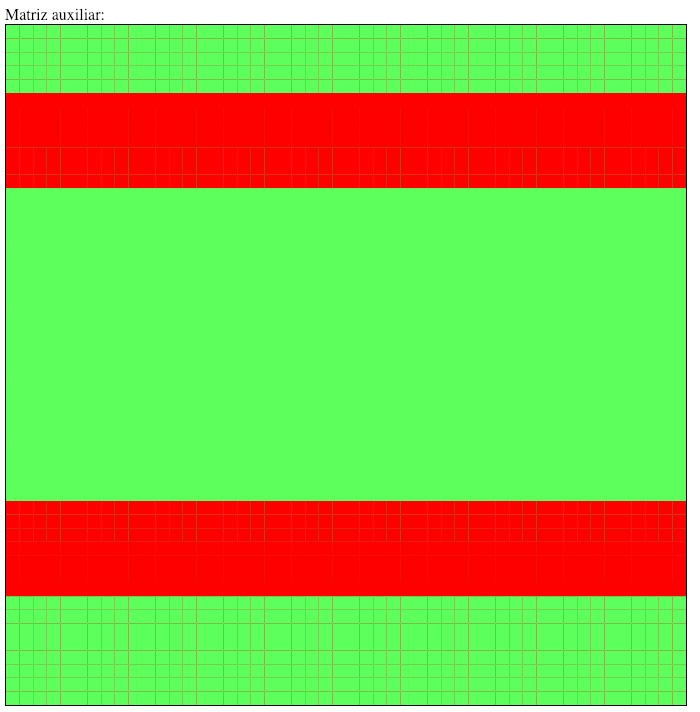
\includegraphics[scale=.3]{GOLM/img/regla3317-2-1.png}
			\caption{Matriz auxiliar}
			\label{fig:golm33}
		\end{center}
	\end{figure}

	Finalmente, al usar la función de paridad, se obtiene algo muy interesante, ya que de igual forma se empieza a formar un mosaico, pero las formas dentro de este son muy curiosas, ya que son figuras geométricas complejas que hasta el momento no había visto en otro autómata.
	\begin{figure}[H]
		\begin{center}
			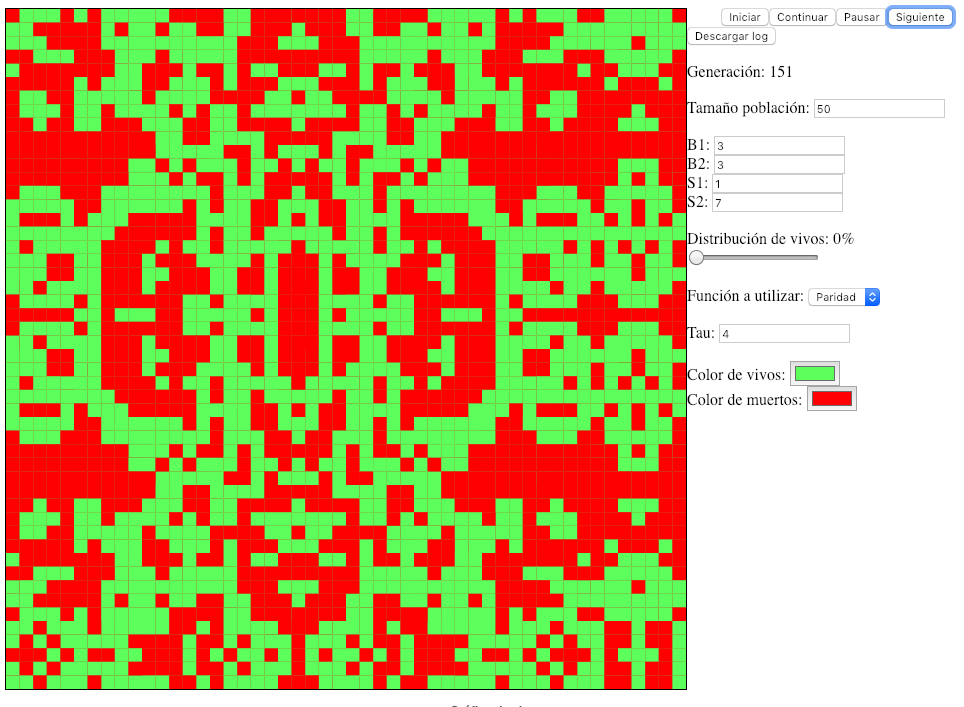
\includegraphics[scale=.3]{GOLM/img/regla3317-3.png}
			\caption{Resultado de iterar usando función de paridad}
			\label{fig:golm34}
		\end{center}
	\end{figure}

	la matriz auxiliar de este autómata, igualmente forma un mosaico con colores invertidos.
	\begin{figure}[H]
		\begin{center}
			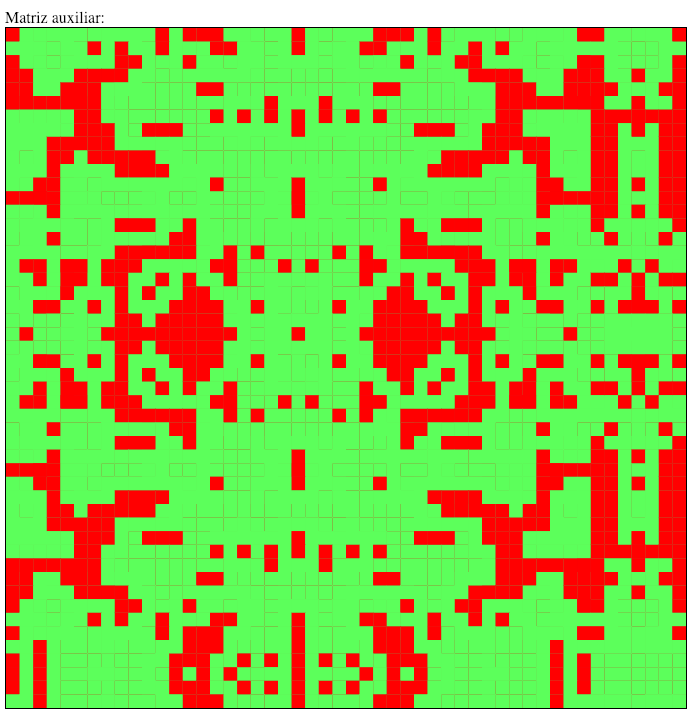
\includegraphics[scale=.3]{GOLM/img/regla3317-3-1.png}
			\caption{Matriz auxiliar}
			\label{fig:golm35}
		\end{center}
	\end{figure}

